\hypertarget{pclCloudViewer_8cpp}{}\section{/home/viki/catkin\+\_\+ws/src/\+Robotic-\/polishing/src/pcl\+\_\+midterm/pcl\+Cloud\+Viewer.cpp File Reference}
\label{pclCloudViewer_8cpp}\index{/home/viki/catkin\+\_\+ws/src/\+Robotic-\/polishing/src/pcl\+\_\+midterm/pcl\+Cloud\+Viewer.\+cpp@{/home/viki/catkin\+\_\+ws/src/\+Robotic-\/polishing/src/pcl\+\_\+midterm/pcl\+Cloud\+Viewer.\+cpp}}


This is the implementation of the \hyperlink{classpclCloudViewer}{pcl\+Cloud\+Viewer} class. This class consists of 1 method. Please refer the \hyperlink{pclCloudViewer_8h}{pcl\+Cloud\+Viewer.\+h} for more detail.  


{\ttfamily \#include $<$pcl/visualization/cloud\+\_\+viewer.\+h$>$}\\*
{\ttfamily \#include $<$pcl/io/io.\+h$>$}\\*
{\ttfamily \#include $<$pcl/io/pcd\+\_\+io.\+h$>$}\\*
{\ttfamily \#include $<$pcl/point\+\_\+types.\+h$>$}\\*
{\ttfamily \#include \char`\"{}pcl\+Cloud\+Viewer.\+h\char`\"{}}\\*
{\ttfamily \#include $<$iostream$>$}\\*
Include dependency graph for pcl\+Cloud\+Viewer.\+cpp\+:
\nopagebreak
\begin{figure}[H]
\begin{center}
\leavevmode
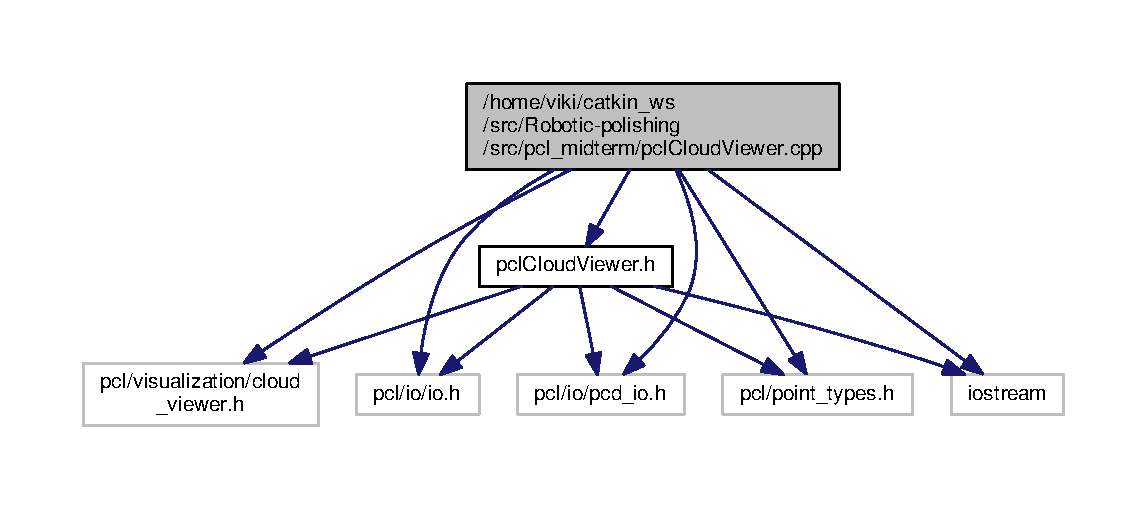
\includegraphics[width=350pt]{pclCloudViewer_8cpp__incl}
\end{center}
\end{figure}


\subsection{Detailed Description}
This is the implementation of the \hyperlink{classpclCloudViewer}{pcl\+Cloud\+Viewer} class. This class consists of 1 method. Please refer the \hyperlink{pclCloudViewer_8h}{pcl\+Cloud\+Viewer.\+h} for more detail. 

\begin{DoxyAuthor}{Author}
Michael Kam (michael081906) 
\end{DoxyAuthor}
\begin{DoxyRefDesc}{Bug}
\item[\hyperlink{bug__bug000029}{Bug}]No known bugs. \end{DoxyRefDesc}
\begin{DoxyCopyright}{Copyright}
G\+NU Public License.
\end{DoxyCopyright}
This class utilize pcl visualization to display point cloud.

\begin{DoxyAuthor}{Author}
Michael Kam (michael081906) 
\end{DoxyAuthor}
\begin{DoxyRefDesc}{Bug}
\item[\hyperlink{bug__bug000030}{Bug}]No1 can\textquotesingle{}t not be compile successfully in the test case. \end{DoxyRefDesc}
\begin{DoxyCopyright}{Copyright}
G\+NU Public License.
\end{DoxyCopyright}
\hyperlink{classpclCloudViewer}{pcl\+Cloud\+Viewer} is free software\+: you can redistribute it and/or modify it under the terms of the G\+NU General Public License as published by the Free Software Foundation, either version 3 of the License, or (at your option) any later version.

\hyperlink{classpclCloudViewer}{pcl\+Cloud\+Viewer} is distributed in the hope that it will be useful, but W\+I\+T\+H\+O\+UT A\+NY W\+A\+R\+R\+A\+N\+TY; without even the implied warranty of M\+E\+R\+C\+H\+A\+N\+T\+A\+B\+I\+L\+I\+TY or F\+I\+T\+N\+E\+SS F\+OR A P\+A\+R\+T\+I\+C\+U\+L\+AR P\+U\+R\+P\+O\+SE. See the G\+NU General Public License for more details. You should have received a copy of the G\+NU General Public License along with \hyperlink{classpclCloudViewer}{pcl\+Cloud\+Viewer}. If not, see \href{http://www.gnu.org/licenses/}{\tt http\+://www.\+gnu.\+org/licenses/}. $\ast$ 